\documentclass[11pt]{amsart}
\usepackage{amstext,amsfonts,amssymb,amscd,amsbsy,amsmath,verbatim, mathrsfs, fullpage}
\usepackage[alphabetic,abbrev,lite]{amsrefs} % for bibliography 
%\usepackage{ifthen,tikz}
%\usepackage{tikz-cd}
\usepackage{diagrams}
\usepackage[dvipsnames]{xcolor}
\usepackage{tikz}
\usetikzlibrary{arrows, shapes, positioning, calc, patterns, cd}

\usepackage{color}
\usepackage{amsthm}
\usepackage{latexsym}
\usepackage[color, matrix, arrow]{xy}
\usepackage{enumerate}
\usepackage{mathtools,accents}
\setcounter{MaxMatrixCols}{15}


\DeclarePairedDelimiter\ceil{\lceil}{\rceil}
\DeclarePairedDelimiter\floor{\lfloor}{\rfloor}

\numberwithin{equation}{section}

\newtheorem{lemma}[equation]{Lemma}
\newtheorem{theorem}[equation]{Theorem}
\newtheorem*{gr}{Green's Linear Syzygy Theorem}
\newtheorem{propo}[equation]{Proposition}
\newtheorem{prop}[equation]{Proposition}
\newtheorem{cor}[equation]{Corollary}
\newtheorem{conj}[equation]{Conjecture}
\newtheorem{claim}[equation]{Claim}
%\newtheorem{claim*}{Claim}
\newtheorem{thm}[equation]{Theorem}
\newtheorem{convention}[equation]{Convention}
\newtheorem{question}[equation]{Question}


\theoremstyle{definition}
\newtheorem{defn}[equation]{Definition}
\newtheorem{example}[equation]{Example}
\newtheorem{notation}[equation]{Notation}
\newtheorem{construction}[equation]{Construction}
\newtheorem{algorithm}[equation]{Algorithm}
\newtheorem{warning}[equation]{Warning}
\newtheorem{conventions}[equation]{Conventions}

\theoremstyle{remark}
\newtheorem{remark}[equation]{Remark}
\newtheorem{remarks}[equation]{Remarks}
\newtheorem{rem}[equation]{Remark}
\newtheorem*{claim*}{Claim}
\newtheorem*{case*}{Case}

% Commands

\newcommand{\Kos}{\mathcal{K}}
\newcommand{\cS}{\mathcal{S}}
\newcommand{\rC}{\mathrm{C}}
\newcommand{\Cech}{\check{\mathrm{C}}}
\newcommand{\Tate}{\on{Tate}}
\newcommand{\Tail}{{\mathbf{Tail}}}
\newcommand{\cC}{\mathcal{C}}
\newcommand{\cK}{\mathcal{K}}
\newcommand{\tot}{\operatorname{tot}}

\newcommand{\isom}{\cong}
\newcommand{\m}{\mathfrak m}
\newcommand{\PP}{\mathbb P}
\newcommand{\PPv}{\mathbb P_{\on{var}}}
\newcommand{\bD}{\mathbf D}
\newcommand{\df}{\operatorname{diff}}
\renewcommand{\P}{\PP}
\newcommand{\bA}{\mathbb A}
\newcommand{\A}{\bA}
\newcommand{\HH}{\mathrm H}
\newcommand{\GG}{\mathbb G}
\newcommand{\ZZ}{\mathbb Z}
\newcommand{\QQ}{\mathbb Q}
\newcommand{\RR}{\mathbb R}
\newcommand{\bH}{\mathbf H}
\newcommand{\bF}{\mathbf F}
\newcommand{\DD}{\mathbf D}
\newcommand{\lideal}{\langle}
\newcommand{\rideal}{\rangle}
\newcommand{\initial}{\operatorname{in}}
\newcommand{\pdim}{\operatorname{pdim}}
\newcommand{\Hilb}{\operatorname{Hilb}}
\newcommand{\Spec}{\operatorname{Spec}}
%\newcommand{\NE}{\overline{\operatorname{NE}}}
\newcommand{\Eff}{\operatorname{Eff}}
\newcommand{\im}{\operatorname{im}}
\newcommand{\NS}{\operatorname{NS}}
\newcommand{\Frac}{\operatorname{Frac}}
\newcommand{\ch}{\operatorname{char}}
\newcommand{\Proj}{\operatorname{Proj}}
\newcommand{\id}{\operatorname{id}}
\newcommand{\Div}{\operatorname{Div}}
\newcommand{\tr}{\operatorname{tr}}
\newcommand{\Tr}{\operatorname{Tr}}
\newcommand{\Supp}{\operatorname{Supp}}
\newcommand{\Gal}{\operatorname{Gal}}
\newcommand{\Pic}{\operatorname{Pic}}
\newcommand{\QQbar}{{\overline{\mathbb Q}}}
\newcommand{\Br}{\operatorname{Br}}
\newcommand{\Bl}{\operatorname{Bl}}
\newcommand{\Cox}{\operatorname{Cox}}
\newcommand{\Tor}{\operatorname{Tor}}
\newcommand{\diam}{\operatorname{diam}}
\newcommand{\Hom}{\operatorname{Hom}} %done
\newcommand{\sheafHom}{\mathcal{H}om}
\newcommand{\Gr}{\operatorname{Gr}}
\newcommand{\HF}{\operatorname{HF}}
\newcommand{\HP}{\operatorname{HP}}
\newcommand{\Osh}{{\mathcal O}}
\newcommand{\cO}{{\mathcal O}}
\newcommand{\kk}{{\bf k}}
\newcommand{\rank}{\operatorname{rank}}
\newcommand{\length}{\operatorname{length}}
\newcommand{\codim}{\operatorname{codim}}
\newcommand{\depth}{\operatorname{depth}}
%\newcommand{\FF}{\mathbb{F}}
\newcommand{\F}{\FF}
\newcommand{\Sym}{\operatorname{Sym}} %done
\newcommand{\GL}{{GL}}
\newcommand{\R}{\mathbb{R}}
\newcommand{\CC}{\mathbb{C}}
\newcommand{\Syz}{\operatorname{Syz}}
\newcommand{\Prob}{\operatorname{Prob}}
\newcommand{\defi}[1]{\textsf{#1}} % for defined terms
\newcommand{\Htot}{H_{\tot}}
\newcommand{\Ltot}{L_{\tot}}
\newcommand{\beq}{\begin{displaymath}}
\newcommand{\eeq}{\end{displaymath}}
\newcommand{\bs}{\backslash}
\newcommand{\ff}{\mathbf{f}}
\newcommand{\Gam}{\Gamma}
\newcommand{\Lotimes}{\overset{L}{\otimes}}
\newcommand{\uHom}{\underline{\Hom}}
\def\nc{\newcommand}
\nc{\tors}{\on{tors}}



\newcommand{\Bmod}{\ensuremath{B_\text{mod}}}
\newcommand{\Bint}{\ensuremath{B_\text{int}}}
\newcommand\commentr[1]{{\color{red} \sf [#1]}}
\newcommand\commentb[1]{{\color{blue} \sf [#1]}}
\newcommand\commentm[1]{{\color{magenta} \sf [#1]}}
\newcommand{\daniel}[1]{{\color{blue} \sf $\clubsuit\clubsuit\clubsuit$ Daniel: [#1]}}
\newcommand{\michael}[1]{{\color{red} \sf $\clubsuit\clubsuit\clubsuit$ Michael: [#1]}}
\newcommand{\maya}[1]{{\color{green} \sf $\clubsuit\clubsuit\clubsuit$ Maya: [#1]}}

\def\edim{\operatorname{edim}}
\def\reg{\operatorname{reg}}

\newcommand{\ve}[1]{\ensuremath{\mathbf{#1}}}
\newcommand{\chr}{\ensuremath{\operatorname{char}}}

%Added by MB:
\def\nc{\newcommand}
\def\on{\operatorname}
%\nc{\Q}{\mathbb{Q}}
%\nc{\RR}{\mathbf{R}}
\nc{\LL}{\mathbf{L}}
\nc{\xra}{\xrightarrow}
\nc{\xla}{\xleftarrow}
\def\a{\mathbf{a}}
\def\om{\omega}
\def\Om{\Omega}
\def\DM{\operatorname{DM}}
\def\Coh{\operatorname{Coh}}
\def\Mod{\operatorname{Mod}}
\def\free{\operatorname{free}}
\def\QCoh{\operatorname{QCoh}}
\def\Cpx{\operatorname{Cpx}}
\def\th{\on{th}}
\def\F{\mathcal{F}}
\def\coker{\on{coker}}
\def\p{\partial}
\def\wt{\widetilde}
\def\i{\iota}
\nc{\into}{\hookrightarrow}
\nc{\onto}{\twoheadrightarrow}
\nc{\OO}{\mathcal{O}}
\nc{\Z}{\mathbb{Z}}
\nc{\cA}{\mathcal{A}}
\nc{\w}{\widehat}
\nc{\End}{\on{End}}
\nc{\res}{\frac{1}{x_0x_1}}
\nc{\tF}{\widetilde{F}}
\nc{\tG}{\widetilde{G}}
\nc{\tf}{\widetilde{f}}
\nc{\Com}{\on{Com}}
\nc{\exact}{\on{exact}}

\nc{\G}{\mathbb{G}}
\nc{\cG}{\mathcal{G}}
\nc{\cE}{\mathcal E}
\nc{\cF}{\mathcal F}
\nc{\cR}{\mathcal R}
\nc{\cD}{\mathcal D}
\nc{\cB}{\mathcal B}
\nc{\cT}{\mathcal T}
\nc{\cL}{\mathcal L}
\def\M{\mathcal{M}}
\nc{\bM}{\mathbf M}
\nc{\bN}{\mathbf N}
\nc{\U}{\mathbf U}
\nc{\BM}{\mathbf B \mathbf M}
\nc{\Dsg}{\on{D}_{\on{sg}}}
\nc{\fC}{\mathcal{C}}
\nc{\fG}{\mathcal{G}}
\nc{\N}{\mathbb{N}}



%When merging files, add these
\nc{\del}{\partial}
\nc{\cone}{\on{cone}}
\nc{\D}{\on{D}_{\on{diff}}}
\nc{\DMb}{\on{D}^b_{\DM}}
\nc{\Db}{\on{D}^{\on{b}}}
\nc{\Kb}{\on{K}^{\on{b}}}
\nc{\fm}{\mathfrak{m}}
\nc{\Flag}{\on{Flag}}
\nc{\DMmin}{\DM_{\on{min}}}
\nc{\Ddiff}{\on{D}_{\on{diff}}}
\nc{\Dbdiff}{\on{D}^\on{b}_{\on{diff}}}
\nc{\wO}{\widehat{\OO}}
\nc{\wT}{\widehat{T}}
\nc{\from}{\leftarrow}
\nc{\wLL}{\widetilde{\LL}}
\nc{\augCech}{\widetilde{\cC}}
\nc{\Fold}{\on{Fold}}
\nc{\Ext}{\on{Ext}}
\nc{\RHom}{\on{RHom}}
\nc{\FF}{\mathbf{F}}
\nc{\Comper}{\Com_{\on{per}}}
\nc{\Unfold}{\on{Unfold}}
\nc{\intHom}{\underline{\Hom}}
\nc{\Ex}{\on{Ex}}
\nc{\tg}{\widetilde{g}}
\def\tP{\widetilde{P}}
\def\b{\beta}
\nc{\B}{\mathcal{B}}
\nc{\K}{\mathcal{K}}
\nc{\kos}{\on{Kos}}
\nc{\Perf}{\on{Perf}}
\nc{\tR}{\widetilde{\cR}}
\nc{\X}{\mathcal{X}}
\nc{\Cl}{\on{Cl}}
\nc{\fU}{\mathcal{U}}
\nc{\bU}{\mathbf U}
\def\co{\colon}
\def\ce{\coloneqq}
\nc{\st}{\on{st}}
\def\E{\mathcal{E}}
\nc{\coh}{\on{coh}}
\def\ex{\on{ex}}
\def\D{D}
\def\lin{\on{lin}}
\def\g{\gamma}
\nc{\tU}{\U}
\nc{\bC}{\mathbf{C}}
\nc{\aux}{\on{aux}}
\def\d{\mathbf{d}}
\def\phi{\varphi}
\def\cP{\mathcal{P}}
\def\I{\mathcal{I}}
\def\geo{\on{geo}}
\def\T{\mathbf{T}}
\nc\Dsing{\on{D}^{\on{sing}}}
\def\Y{\mathcal{Y}}
\def\bL{\mathbf{L}}
\def\k{\mathbf{k}}
\def\e{\epsilon}
\def\epsilon{\varepsilon}
\def\w{\mathbf w}
\def\colim{\on{colim}}
\def\fix#1{{{\bf ***}#1{\bf ***}}}
%\title[Toric methods in homological algebra]{Arbeitsgemeinschaft:  \\ Toric methods in homological algebra \\ October 11 - 16, 2026}
\title[New homological methods in toric geometry]{Notes for Arbeitsgemeinschaft:  \\ New homological methods in toric geometry}
\author{Michael K. Brown}
\author{David Eisenbud}
\author{Daniel Erman}
%This command gets rid of the MR number in the bibliography
\def\MR#1{}

\begin{document}
    \maketitle

\section{Good multigradings}
We let $S=k[x_1, \dots, x_n]$ be a polynomial ring and we will use $\Cl(S)$ to denote an arbitrary finitely generated abelian group.  We will consider $S$ as graded with respect to $\Cl(S)$ via a map $\ZZ^n\overset{\deg}{\longrightarrow}\Cl(S)$ where $\epsilon_1, \dots, \epsilon_n$ are a fixed basis of $\ZZ^n$ and where we set $\deg(x_i) :=\deg(\epsilon_i)\in \Cl(S)$.  
To avoid trivialities, we will always assume that the map $\deg$ is surjective.

Our goal in this section is to articulate conditions under which the multigraded ring $S$ corresponds to the Cox ring of some projective toric variety.

We will need some notation.  We write $M:=\ker(\deg)$ and we consider the induced short exact sequence:
\[
0\to M\overset{\alpha}{\to} \ZZ^n \overset{\deg}{\longrightarrow} \Cl(S) \to 0.
\]
We will define $\Eff(S) :=\{d \in \Cl(S) | S_d \ne 0\}$.  We refer to this as the \defi{effective semigroup} as it forms a subsemigroup of $\Cl(S)$.  We can consider the corresponding cone $\Eff(S)_{\QQ}\subseteq \Cl(S)\otimes_{\ZZ}\QQ$ which is the positive rational cone spanned by the image of $\Eff(S)$ under the natural map to $\Cl(S)\otimes_{\ZZ}\QQ$.


\begin{defn}\label{defn:posGrading}
    We say that $S$ is a \defi{positively graded ring} if there exists a group homomorphism $\phi\colon \Cl(S) \to \ZZ$ such that $\phi \circ \deg(\epsilon_i) > 0 $ for all $i$.
\end{defn}
\begin{lemma}
The following are equivalent:
\begin{enumerate}
    \item $S$ is positively graded.
    \item $S_0=k$.
    \item $\Eff(S)_{\QQ}$ is a pointed cone.
\end{enumerate}
\end{lemma}
\begin{proof}
(1) implies (2) is easy.

For (2) implies (3):  If $\Eff(S)_{\QQ}$ is not a pointed cone then there exist $d\in \Cl(S)$ with $d\neq 0$ where $d$ and $-d$ both lie in $\Eff(S)$. If $S_0\ne k$ then, since $S$ is a domain whose only units are the 
scalars, we must have $d=0$, a contradiction.

For (3) implies (1):  Define the positive grading $\phi$ by choosing a vector space $\Cl(S)\otimes \QQ\to \QQ$ that sends $\Eff(S)_{\QQ}$ into $\QQ_{>0}$ and then clearing denominators as needed
\end{proof}

\begin{prop}
The following are equivalent:
\begin{enumerate}
 \item There is a polynomial ring $S$, graded via $\deg\colon \ZZ^n\to \Cl(S)$, that satisfies the following conditions:
    \begin{enumerate}
        \item $\deg$ is surjective;
        \item $S$ is positively graded;
        \item Each row of $\alpha$ is the primitive point on a distinct ray; that is, the rows of
        $\alpha$ are distinct, nonzero, and have greatest common divisor 1.
        %matrix representing $\alpha\colon M\to \ZZ^n$ has no zero rows and no rows that are scalar multiples of one another.
    \end{enumerate}
    \item There is a simplicial, projective toric variety $X$ with $\Cl(X) = \Cl(S)$ and where the Cox ring of $X$ equals $S$.
\end{enumerate}
\end{prop}
\begin{proof}
    (2) implies (1) is easy.  Given such an $X$ we start choose a basis for the lattice $N$ and take the corresponding basis for the dual lattice $M$.  Since the Cox ring of $X$ is $S$, we know that $X$ involes $n$ rays, and so we have the matrix of rays $N\gets \ZZ^n$.  Since the rays are distinct (and nonzero) the columns of this matrix all nonzero and are not scalar multiples of one another. Dualizing this then yields a map $\alpha\colon M\to \ZZ^n$ satisfying condition (iii).  We set $\Cl(S):=\Cl(X)$ and the induced grading satisfies (i) and (ii) by standard facts.
    
    (1) implies (2) is more subtle.  The $\Cl(S)$-grading on $S$ induces a GIT problem and hence a secondary fan.  If $X_{\Sigma}$ is the toric variety associated to some of the secondary fan, Proposition 14.4.1 (a basic fact on Gale duality) implies that the support of the fan $\Sigma$ is the cone spanned by the rays in $N_{\QQ}$.

    \begin{lemma}[CLS 14.3.2 without the extra notation]
     Fix a basis $\epsilon$ of $\RR^n$, and let
     \begin{tikzcd}     
    0\arrow{r} &M_\RR^* \arrow{r}{\delta} & \RR^n \arrow{r}{\nu}&N_\RR \arrow{r}&0
    \end{tikzcd}
    be an exact sequence of real vector spaces. If every element of $\epsilon$ maps
    to a nonzero element of $N_\RR$ then $ cone(\nu(\epsilon)) = N_\RR$
    if and only if $cone(\delta^*(\epsilon))$ is pointed.
    \end{lemma} 
    In particular, any $X_{\Sigma}$ from the secondary fan will be proper.

    \def\Eff{{\rm Eff}}
    
    \begin{proof}[Proof of the Lemma] Set $C_\nu :=cone(\nu(\epsilon))$ and
    $\Eff := cone(\delta^*(\epsilon))$. We will prove the contrapositive: 
    
    \noindent $\Rightarrow$: Suppose that $C_\nu = N_\RR$, so $C_\nu^\vee = 0$.
    Suppose that both $v$ and $-v$ are non-negative combinations of the rays
    of $\Eff$. Adding the expressions for these vectors, we get a map $\RR \to \RR^n$ that has non-negative coefficients
    with respect to $\epsilon$, and whose image is in the kernel of $\delta^*$.
    Thus it factors through $N_\RR^*$. Dualizing, we get a functional on
    $N_\RR$ that is non-negative on every ray; that is an element
    of $C_\nu^\vee$. Thus $v = 0$, proving that $\Eff$ is pointed.
  
    \noindent $\Leftarrow$: Conversely, if $\Eff$ is pointed then there
    is a map $M_\RR \to \RR$ that is positive on every ray of $C_\nu$. Dualizing, we get an
    element $w \in \ker \nu$ with all positive coefficients. If $\phi: N_\RR \to \RR$
    is an element of $C_\nu^\vee$, then, because all the rays of $N_R$ are nonzero, $\phi(w)=0$ is a positive combination of some of the coefficients of $w$. Thus $C_\nu^\vee = 0$ and $C_\nu = C_\nu^{\vee\vee} = N_\RR$.
    \end{proof}
    
    % We find the rays by dualizing the map $\alpha\colon M\to \ZZ^n$ obtaining $\alpha^*\colon \ZZ^n \to N$.  So we need to show that the positive rational cone spanned by the columns of $\alpha^*$ in $N_{\QQ}$ is the entire space.  Choose $\phi$ as in Definition~\ref{defn:posGrading}.  We get a new exact sequence
%    \[
 %   0\to M'\overset{\gamma}{\to} \ZZ^n \overset{\phi\circ \beta}{\to} \ZZ\to 0.
 %   \]
  %  Because we have a positive grading, the map $\ZZ^n\to \ZZ$ has the form $(a_1, \dots, a_n)$ for positive integers $a_i\in \ZZ_{>0}$ and we can explicitly compute the kernel as 
   %%\begin{pmatrix}
     %   -a_2&-a_3&\cdots &-a_n\\
      %  a_1&0&\cdots &0\\
       % 0&a_1&\cdots &0\\
       % 0&0&\cdots &a_1
   % \end{pmatrix}
   % \]
   % The cone over the rows of $\gamma$ fills an entire $\QQ^{n-1}$.  And the cone over the rows of $\alpha$ is a projective of that cone under a map $\QQ^{n-1} \to N\otimes \QQ$ and hence we obtain the desired result.

    Proposition 14.4.1 also implies that each $X_{\Sigma}$ is semiprojective and since it is proper by the previous paragraph, it is also projective.
    
   We next utilize Proposition 15.1.6 of CLS.  This says that we have a chamber of the secondary fan where the corresponding variety $X_{\Sigma}$ requires $n$ rays if and only if the rows of $\alpha$ are nonzero and generate distinct rays, which is implied by condition (c).  In this case, $\alpha^*: \ZZ^n\to N$ will determine the rays of $X_{\Sigma}$.  The stronger condition, that the rows of $\alpha$ each represent a primitive point on a distinct ray, then implies that the ray matrix for $X_{\Sigma}$ will be precisely $\alpha^*$.  Since the Class group of $X$ is computed in terms of the ray matrix, we have that the class group of $X$ will equal $\Cl(S)$, and the map $\ZZ^{n}\to \Cl(X)$ will agree with the map $\deg$.  Thus the Cox ring of $X_{\Sigma}$ will be a polynomial ring on $n$ variables and the grading will be as desired.
\end{proof}

\section{Equivalent conditions for Bondal-Thomsen}

The Bondal-Thomsen collection is a finite set of line bundles that can be defined in several different ways.  We will take the following definition, originally due to Bondal, as our definition.  Consider the short exact seuqence
\[
0\to M\overset{\alpha}{\longrightarrow} \ZZ^n \overset{\deg}{\longrightarrow} \Cl(X) \to 0.
\]
We write $\alpha_\rho$ for the projection of $\alpha$ onto the basis vector corresponding to $\rho$ in $\Sigma(1)$.   (Explicitly we have $\alpha_\rho(m) = \langle -m, u_\rho\rangle$ in the standard notation of CLS, but I don't think this is actually so relevant.)
Identifying $\ZZ^n$ with torus invariant divisors, we explictly have $\alpha(m) = \sum_{\rho} \alpha_\rho(m) D_\rho$ and the class of $\alpha(m)$ is $0$ in $\Cl(X)$ for all $m\in M$.

We now extend this to $M\otimes \QQ$ as follows.  We write $\alpha\otimes {\QQ}$ for the corresponding map of vector spaces $M\otimes \QQ\to \QQ^n$.  And we will write $\lfloor \alpha \rfloor$ for the map
\[
\lfloor \alpha \rfloor\colon M\otimes \QQ \to \ZZ^n \text{ where } m\mapsto \sum_{\rho} \lfloor \alpha_\rho(m) \rfloor D_\rho.
\]
We note that, while $\alpha(m)$ will always be trivial as an element of $\Cl(X)\otimes \QQ$, this is not the case for $\lfloor \alpha \rfloor(m)$.   

\begin{defn}\label{defn:BTcollection}
    The \defi{Bondal-Thomsen collection} $\Theta_X\subseteq \Cl(X)$ is the image of $\deg \circ \lfloor \alpha \rfloor$.  
    %In other words, an element $d\in \Cl(X)$ lies in The Bondal-Thomsen collection if and only if there is some $m\in M\otimes \QQ$ such that $\lfloor \alpha \rfloor(m)$ is linearly equivalent (as $\QQ$-divisors) to the (honest, i.e. non $\QQ$-divisor) $d\in \Cl(X)$.
\end{defn}
Note that, since the sublattice $M\subseteq M\otimes \QQ$ maps to $0$ in $\Cl(X)$, it would be equivalent to consider points in the rational torus $M\otimes \QQ / M$.

\begin{example}
    Let $X=\PP^2$.  Then $M=\ZZ^2$ and $\alpha$ is given by the matrix
    \[
    \begin{pmatrix}
        1&0\\ 0&1\\-1&-1
    \end{pmatrix}
    \]
    Since it suffices to consider points in $M\otimes \QQ / M$, it suffices to consider $(a,b)\in M\otimes \QQ^2$ where $0\leq a,b <1$.  In this case we have
    \[
    \lfloor \alpha \rfloor (a,b) = \lfloor -a\rfloor D_0 + \lfloor -b\rfloor D_1 + \lfloor a+b \rfloor D_2.
    \]
    Since all the prime torus divisors $D_0,D_1,D_2$ are equivalent to $\cO_{\PP^2}(1)$, determining the Bondal-Thomsen collection for $\PP^2$ amounts to answering: which integers can arise as a sum
    \[
    \lfloor -a\rfloor + \lfloor -b\rfloor + \lfloor a+b\rfloor \text{ with } (a,b) \in [0,1)^2.
    \]
    If $(a,b)=(0,0)$ we get $0$.  If $0<a<1$ and $b=0$ or vice versa, we get $-1$. $0<a<1$ and $0<b<1$ and $a+b<1$ then we get $-2$, otherwise we get $-1$.  In particular, we conclude that the Bondal-Thomsen collection is $\cO,\cO(-1),\cO(-2)$ in this case.
\end{example}

\begin{defn}\label{defn:KoszulZonotope}
    The \defi{Koszul zonotope} is the locus 
    \[
    \mathcal Z:=\sum_{\rho} a_\rho \deg(x_\rho) \subseteq  \Cl(X)\otimes \QQ\footnote{As a technical note:  when $\Cl(X)$ has torsion, we always consider degrees under the natural map $\Cl(X)\to \Cl(X)\otimes \QQ$.} \text{ with } a_\rho \in (-1,0].
    \]
\end{defn}

\begin{defn}\label{defn:KoszulZonotope}
    The \defi{toric Frobenius map of degree $\ell$} is the morphism $F_{\ell} \colon X\to X$ that is induced by the map of Cox rings $S\to S$ given by sending $x_\rho \mapsto x_\rho^{\ell}$ for all $\ell$.
\end{defn}

\begin{example}
    Continuing the example of $\PP^2$, the zonotope $\mathcal Z$ is simply the half-open interval $(-3,0]$.  Thus the lattice points correspond to $-2,-1$ and $0$.  Moreover, if we consider
\end{example}
\begin{thm}
    The follows subsets of $\Cl(X)$ are all equal to the Bondal-Thomsen collection.
    \begin{enumerate}
        \item  The set of degrees $d\in \Cl(X)$ as in Definition~\ref{defn:BTcollection}.
        \item  The set of degrees $d\in \Cl(X)$ such that: in $\Cl(X)\otimes \QQ$, $d$ is equivalent to an element $\sum_{\rho} a_\rho D_\rho$ with $a_\rho \in (-1,0].$
        \item  The set of degrees $d\in \Cl(X$) such that $\deg_{\QQ}(d)$ lies in the zonotope $\mathcal Z$.
        \item  The set of degrees $d\in \Cl(X$) such that: there is some $\ell>0$, where $\cO_X(d)$ appears as a summand of $F_{\ell,*}\cO_X$.
        \item  The set of degrees $d\in \Cl(X$) such that: for any $\ell\gg 0$, $\cO_X(d)$ appears as a summand of $F_{\ell,*}\cO_X$.
    \end{enumerate}
\end{thm}
\begin{proof}
(1) $\Rightarrow$ (2):
Let $m \in M\otimes \QQ$.  Consider the difference
\[
\lfloor \alpha \rfloor(m) - \alpha(m) = \sum_{\rho} \left(\lfloor \alpha_\rho(m) \rfloor - \alpha_\rho(m)\right) D_\rho.
\]
But for any rational number $z$, the difference between $\lfloor z\rfloor$ and $z$ lies in $(-1,0]$ and ehnce this divisor has the desired form.  Since $\alpha(m)$ is trivial in $\Cl(X)\otimes \QQ$ we have the desired result.


(2) $\iff$  (3) is trivial.

(2) $\iff$ (4) $\iff$ (5) appear in~\cite[Theorem 2]{achinger}, in the case $D=0$.
\end{proof}

One important fact about the Bondal-Thomsen collection is the following easy consequence of Demazure Vanishing.

\begin{prop}
    Let $a\in \Cl(X)$ correspond to an ample class and let $d\in \Cl(X)$ corresponds to an element of the Bondal-Thomsen collection $\Theta$.  Then 
    \[
    H^i(X,\cO_X(a+d)) = 0 \text{ for all } i>0.
    \]
\end{prop}

\begin{comment}
    
Claim:
There are 4 ways to think about the Bondal-Thomsen collection which we claim are all equivalent.

(1)  Via Bondal’s definition, i.e. as the image in Cl(X) of the map M\otimes \RR —> Cl(X) where the point \theta maps via the round-down formula in Definition 2.12 as in our King paper.  Specifically we send \theta \mapsto D(\theta) := \sum_\rho \lfloor <-\theta, u_\rho> \rfloor D_\rho.

(2)  As the elements in Cl(X) that are linearly equivalent (in Cl(X)\otimes RR) to a RR-divisor of the form \sum_{\rho} a_\rho D_{\rho} with with a_\rho \in (-1,0].

(3)  As the lattice points inside of the zonotope associated to (2).

(4)  As the summands of the pushforward under Frobenius.

Proof:
(2) <==> (3) is obvious.

(1) <==> (2) is as follows.   Let \theta \in M\otimes \RR and D(\theta) as in (1).  Define D’(\theta) by the same formula but without the round down. That is, D’(\theta) = \sum_\rho \lfloor -\theta, u_\rho \rfloor D_\rho is an \RR-divisor which is equivalent to 0 in Cl(X)\otimes RR.  This is because D’(\theta) is the image of \theta under the composition of maps in the exact sequence:

0—> M\otimes RR —> RR^{\Sigma(1)} —> Cl(X)\otimes RR —> 0

Now examine the coefficients of D - D’.  For each \rho, the coefficient of D-D’ is \lfloor <-\theta, u_\rho> \rfloor -  <-\theta, u_\rho>.  But for any real number \zeta, the difference \lfloor \zeta \rfloor - \zeta lies in the range (-1,0].  It follows So D(\theta) - D’(\theta) has the form of a divisor from (2).  Since D’(\theta) is linearly equivalent to 0, we obtain the result.

(2) <==> (4) is from Theorem 2 of Achinger 2015 (the D = 0 case), which is not so bad.

How does this look?
\end{comment}


\begin{comment}
\section{Secondary fan example}


\begin{center}
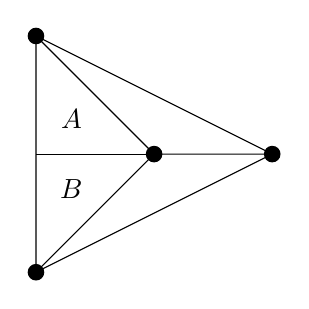
\begin{tikzpicture}[scale=1.5]
    % Define the points for easier reference
    \coordinate (A) at (1,0);
    \coordinate (B) at (2,0);
    \coordinate (C) at (0,1);
    \coordinate (D) at (0,-1);
    \coordinate (E) at (0,0);
    \coordinate (F) at (1.2,0.2);
    \coordinate (G) at (2.2,0.2);
    \coordinate (H) at (0.2,1.2);
    \coordinate (I) at (0.2,-.8);
    \coordinate (J) at (0.2,0.2);

    % Draw all line segments connecting the points
    \draw (A) -- (B) -- (C) -- cycle;
    \draw (A) -- (D) -- (C);
    \draw (B)--(D);
    \draw (A) -- (E);

    % Plot the points (as small black circles)
    \fill (A) circle (2pt);
    \fill (B) circle (2pt);
    \fill (C) circle (2pt);
    \fill (D) circle (2pt);
    \draw (.3,.3) node {$A$};
    \draw (.3,-.3) node {$B$};
\end{tikzpicture}
\end{center}

\end{comment}
\section{Chambers and irrelevant ideals}
%Each point $\mathbf{a} = (a_1, \dots, a_n)\in \ZZ^n$ determines a set of halfspaces in $M\otimes \QQ$ of the form $\alpha_i(m) \geq -a_i$ for $1\leq i \leq n$.  We write $H_{\mathbf{a}} = \cap_{i=1}^n \{\alpha_i(m)\geq -a_i\}$.  The locus $H_{\mathbf{a}}$ will be a convex polytope if and only if the divisor $\sum_{i=1}^n a_iD_i$ is an effective divisor.

%Recall that $r$ is the rank of $\Cl(S)$.  Start with the points $\{ \deg(x_i) \forall 1 \leq i \leq n\}\subseteq \Cl(S)\otimes \QQ$.  

Fix a monomial $\mathbf{x}^{\mathbf{a}}:=x_1^{a_1}\cdots x_n^{a_n}$ and a point $d\in \Cl(S)\otimes \QQ$.  We say that \defi{$\mathbf{x}^{\mathbf{a}}$ spans $d$} if the positive, rational cone spanned by $\{\deg_{\QQ}(x_i) | a_i \ne 0\}$ contains $d$, i.e. if there exist $q_i \in \QQ_{>0}$ such that
$
d = \sum_{a_i \ne 0} q_i\deg_{\QQ}(x_i).
$
This allows us to define a correspondence between convex cones in $\Cl(S)\otimes \QQ$ and squarefree monomial ideals in $S$.  We note that, because we insist that the coefficients $q_i$ be strictly positive, this is an open condition on the points $d$.

\begin{defn}\label{defn:idealConeCorrespondence}
For a convex cone $\Gamma \subseteq \Cl(X)\otimes \QQ$ we define 
    \[
    \text{ideal}(\Gamma):= \langle \mathbf{x}^{\mathbf{a}} | \mathbf{x}^{\mathbf{a}} \text{ spans } d, \forall d\in \Gamma\}.
    \]
    Conversely, given a squarefree monomial ideal $B$ we define 
     \[
    \text{cone}(B):= \{ d | \mathbf{x}^{\mathbf{a}} \text{ spans } d, \forall \mathbf{x}^{\mathbf{a}} \in B\}.
    \]
\end{defn}
Observe that $\text{ideal}(\Gamma)$ is a squarefree monomial ideal in $S$, and $\text{cone}(B)$ is an open convex cone in $\Cl(S)\otimes \QQ$.   Moreover, it is elementary to check that
\[
\text{ideal}(\text{cone}(\text{ideal}(\Gamma))) = \text{ideal}(\Gamma) \qquad \text{ and } \qquad \text{cone}(\text{ideal}(\text{cone}(B))) = \text{cone}(B). 
\]
Since there are only a finite number of squarefree monomial ideals in $S$, it follows that there are a finite list of squarefree monomial ideals $B_1, \dots, B_s$ such that $\text{cone}(B_i)$ is full-dimensional and $\text{ideal}\left(\text{cone}\right)(B_i) = B_i$. We call these cones the \defi{chambers for $S$}.  By definition, the chambers are disjoint from one another.
%By definition, the effective cone is the union of the closures of these chambers.
\begin{defn}\label{defn:chambersIrrelevant}
    To simplify notation, we enumerate the chambers as $\Gamma_1, \dots, \Gamma_s$ and write $B_1, \dots, B_s$ for the corresponding squarefree monomial ideal.
\end{defn}
\begin{remark}
     We will confirm below that each pair $(S,B_i)$ determines a simplicial projective variety $X_i$.  The rough statement is that $X_i$ the quotient $\Spec(S) - V(B_i) / G$ (with the action of $G$ induced by the grading group), but this is a ``rough'' statement because of various subtleties involving quotients of projective varieties.  So there is a sense in which the multigraded ring $S$ naturally corresponds to the set of toric varieties $X_1, \dots, X_r$.

    This connection is even sharper from a homological perspective.  The pair $(S,B_i)$ determines a module category as follows:  we write $\mod(S)$ for the category of $\Cl(S)$-graded $S$-modules and we write $\mod_{B_i}(S)$ for the subcategory  modulo those modules that are annihilated by a power of $B_i$.  To the pair $(S,B_i)$ we can attach the quotient category $\mod(S)/\mod_{B_i}(S)$.  This equals--essentially by defintion--the category of sheaves on the quotient stack $[\Spec(S) - V(B_i)/G]$ which we denote as $\mathcal X_i$.  We will see later that $\mathcal X_i$ is closely related to the aforementioned toric variety $X_i$.
\end{remark}
\begin{cor}
Each $B_i$ is generated by products of $r$ distinct variables.
\end{cor}
\begin{proof}
    Let $x_{i_1}\cdots x_{i_p}$ be a minimal generator of $B_i$ and assume $p>r$.  We have that $\Gamma_i$ is in the span of $\deg_{\QQ}(x_{i_1}), \cdots, \deg_{\QQ}(x_{i_p})$.   Since $\Gamma_i$ is $r$-dimensional, after potentially reindexing, we can assume that $\deg_{\QQ}(x_{i_1}), \cdots \deg_{\QQ}(x_{i_r})$ are linearly independent.  If $\Gamma_i$ lies in the span of these, then $x_{i_1}\cdots x_{i_r}$ lies in $B_i$, contradicting the initial minimal generator assumption.  But then some portion of $\Gamma_i$ would correspond to an ideal containing $x_{i_1}\cdots x_{i_r}$, contradicting the fact that the chambers of squarefree monomial ideals must be disjoint.
\end{proof}
\begin{remark}
By considering intersections of the chambers, we can endow $\Eff(S)$ with a fan structure which is known as the secondary fan.  However, for the applications to Cox categories and King's Conjecture, we do not need the full structure of the secondary fan, we simply need to know the chambers.  So we will omit a fuller discussion of the secondary fan.
\end{remark}
\begin{remark}
    Because each chamber is defined in terms of spanning sets of monomials, the hyperplanes used to define each chamber will have a special form.  Namely, each such hyperplane will be spanned by a codimension $1$ set of linearly independent vectors $\deg_{\QQ}(x_i)$.  
    
    In particular, we can build a naive stratification of $\Eff(X)$ as follows.  Write $r$ for the rank of $\Cl(S)\otimes \QQ$.  For each linearly independent $(r-1)$-tuple of vectors $\deg_{\QQ}(x_i)$, we get a hyperplane, and taking the union of all of these hyperplanes will slice $\Eff(X)$ into a finite set of chambers, each of belongs entirely to one of the chambers $\Gamma_1,\dots, \Gamma_s$.  In particular, the chambers of the secondary fan are a coarsening of the chambers of this naive stratification.
\end{remark}


We can describe the $B_i$ in several equivalent ways.  Recall that we have the map $\deg\colon \ZZ^n\to \Cl(S)$; we write $\deg_{\QQ}$ for the induced map to $\Cl(S)\otimes \QQ$.
\begin{prop}
    Fix a chamber $\Gamma_i$ for $S$ and any ray $\rho \in \Gamma_i$.  The following ideals are equal
    \begin{enumerate}
        \item  The ideal $B_i$ corresponding to $\Gamma_i$, i.e. the ideal $B_{\Gamma_i}$ as in Definition~\ref{defn:idealConeCorrespondence}.
        \item  The $B_{\text{red}}$ radical of the ideal $\langle \mathbf{x}^{\mathbf{a}} \text{ such that } \deg_{\QQ}(\mathbf{x}^{\mathbf{a}})\in \Gamma_i\rangle$.
        \item  The ideal $\sqrt{B_{\rho}}$ defined as the radical of the ideal $\langle \mathbf{x}^{\mathbf{a}} \text{ such that } \deg_{\QQ}(\mathbf{x}^{\mathbf{a}})\in \rho \rangle$
    \end{enumerate}
\end{prop}
\begin{proof}
For (1) $\Rightarrow$ (3): Let $x_{i_1}\cdots x_{i_s}$ be a squarefree monomial which spans $\Gamma_i$.  Since $\rho$ lies in $\Gamma_i$, for some integers $a_1, \dots, a_s$ we have that $\deg_{\QQ}(x_{i_1}^{a_1}\cdots x_{i_s}^{a_s}) \in \rho$.  In particular, $x_{i_1}\cdots x_{i_s}$ belongs to $\sqrt{B_{\rho}}$.

Certainly the ideal from (3) belongs the ideal from (2).

Finally we have (2) $\Rightarrow$ (1):  Let $x_{i_1}, \cdots, x_{i_p}$ be the variables dividing $\mathbf{x}^{\mathbf{a}}$.  Assume, for contradiction, that the corresponding degrees all line on some hyperplane $H$.  Then $H$ subdivides $\Gamma_i$ into two pieces $\Gamma_i^{+}$ and $\Gamma_i^{-}$, corresponding to the two side of $H$.  There must therefore be at least one monomial whose degree lies on either side of $H$, say $\deg_{\QQ}(x_{+})$ is on the $\Gamma_i^{+}$-side and $\deg_{\QQ}(x_{-})$ is on the $\Gamma_i^{-}$-side.  But then the ideals $B_{\Gamma_i^{+}}$ and $\Gamma_i^{-}$ would be distinct, and so $\Gamma_i$ would not be a valid chamber.

We conclude that $\deg_{\QQ}(x_{i_1}), \cdots, \deg_{\QQ}(x_{i_p})$ span an $r$-dimensional cone.  Since this span includes a point in $\Gamma_i$, by construction of the chambers, it must contain the entire chamber $\Gamma_i$.  It follows that $x_{i_1}\cdots x_{i_p}$ lies in $B_i$.
\daniel{This is not well articulated yet, but it's definitely very doable.}
\end{proof}


\subsection{Chambers and toric varieties}
From the irrelevant ideal $B_i$ we can produce a fan $\Sigma_i$ for a toric variety as follows.  We let the rays of $\Sigma_i$ be the set of rays $\rho_j$ such that the corresponding principal ideal $\langle x_j\rangle$ does not contain $B_i$.  And we let the cones of $\Sigma_i$ be the cones spanned by the tuples $\rho_{j_1}, \cdots, \rho_{j_p}$ such that $B_i$ does not contain the monomial $x_{j_1}\cdots x_{j_p}$.    The fans $\Sigma_1, \dots, \Sigma_s$ are all distinct because the $B_i$ are all distinct.

For a point $\mathbf{a}=(a_1, \dots, a_n)\in \ZZ^{n}$ we define the polyhedron
\[
P_{\mathbf{a}} := \cap_{i=1}^n \{ m \in M | \alpha_i(m) \geq -a_i\}.
\]
To a polyhedron $P_{\mathbf{a}}\subseteq M\otimes \QQ$ there is a dual normal fan $\operatorname{NormalFan}(P_{\mathbf{a}})\subseteq N\otimes \QQ$.  We recall that $\operatorname{NormalFan}(P_{\mathbf{a}})\subseteq N\otimes \QQ$ is defined as \dots

The key fact relating these definitions is:
\begin{prop}\label{prop:polytopeAndFan}
We have that $P_{\mathbf{a}}$ is nonempty if and only if $\deg_{\QQ}(\mathbf{a})$ lies in the effective cone.  

Moreover, we have that $\deg_{\QQ}(\mathbf{a}) \in \Gamma_i$ if and only if there is an open neighborhood $U_{\mathbf{a}}$ of $\mathbf{a}$ such that the normal fan of $P_{\mathbf{a'}}$ equals $\Sigma_i$ for all $\mathbf{a}'\in U_{\mathbf{a}}$.
\end{prop}
\daniel{To do:  add references from CLS.}

%In particular, the chambers $\Gamma_i$ also precisely correspond the distinct 


\begin{prop}\label{defn:fanAndXi}
    As defined above we have the following: $\Sigma_i$ is a simplicial fan such that $|\Sigma_i|=N\otimes \QQ$.  In particular,  $\Sigma_i$ is the fan associated to a simplicial, projective toric variety which we denote as $X_i$.
\end{prop}


\begin{lemma}
The following are equivalent:
\begin{enumerate}
    \item The Cox ring of $X_i$ equals $S$;
    \item $\Cl(X_i)=\Cl(S)$;
    \item  The rays of $\Sigma_i$ are precisely $\rho_1, \dots, \rho_n$;
    \item  $B_i$ does not belong to any principal ideal $\langle x_j\rangle$.
\end{enumerate}
\end{lemma}
When these conditions are satsified, the ample cone equals $\Gamma_i$.  \daniel{When these conditions are not satisfied, one needs to be a bit more careful in relating the ample cone with $\Gamma_i$.}


\subsection{Irrelevant ideals for faces of secondary fan}
\daniel{Not sure what we want to put here.}
\begin{lemma}
    For a face of the secondary fan, the irrelevant ideal is the sum irrelevant ideals of the chambers with that face in its boundary.
\end{lemma}

\section{Binomial Ideals and Cellular Resolutions}
Notes on the paper of Berkesch, Heller, Smith, and Yang \cite{BCHSY}.
\medskip

\noindent\emph{Summary} An inclusion $X \to Y$ of toric varieties corresponds to a binomial prime ideal $I$ in the Cox ring $S$ of $Y$, and the
sheafification of $I$ is the ideal sheaf of the subvariety. The paper \cite{BCHSY}  provides an explicit (generally non-minimal) $S$-free resolution of the normalization of the ring $S/I$ in terms of a natural but generally non-integral stratification of the real torus corresponding to $Y$. 

\subsection{Prime binomial ideals}
Binomial ideals in general were studied in \cite{Eisenbud-Sturmfels}. Here is the description of prime binomial ideals from that paper: 

Let $M$ be the set of monomials in $S$, and $\ZZ M$ the associated lattice (free $\ZZ$-module). Any homogeneous  prime binomial ideal $I$ in $S$ corresponds to 
a saturated sublattice $L\subset \ZZ M$ and a character $\rho: L\to \G_{m}$: the set of binomial elements of $I$
expressed in the quotient field of $S$, is
$$
\{\ell - \rho(\ell \mid \ell \in L\}
$$
and thus, clearing denominators and writing $x = x_{0}\dots, x_{n}$ for the generators of $M$, the binomial prime ideal is
$$
I = \{x^{a} -\rho(c) x^{b} \mid c = a-b \in L\}.
$$
In the special case studied in \cite{BCHSY} the character $\rho$ is taken to be the constant function 1, since that is the case required for the toric application.

The ideal $I$ may also be expressed as the kernel of the map sending the $x_{i}$ to
the corresponding (Laurent) monomials in $\ZZ M/\ZZ L$. Thus  $S/I$ is the ring generated by these monomials. The convex hull 
of the rays they generate in $\RR M/\RR L$ form a pointed cone, and the normalization
of $S/I$ is easily seen to be the intersection of this pointed cone with 
$\ZZ M/\ZZ L$; see for example Exercise **** of \cite{EisenbudCA}. (One could just as well use $\QQ M/\QQ L$ everywhere here.) This is a submodule of the quotient field
of $/I$, generated by monomials -- in short a ``monomial module''. It is this, as a module over $S$, that is resolved by the construction of \cite{BCHSY}.

\section{Cellular Resolutions}
\subsection{Revisiting the Koszul complex}
To start with the simplest case: one way to understand the Koszul complex
$\K := K(x_{0}, \dots, x_{n})$ is as a ``homogenization'' of the chain complex of
an $n$-simplex $\Delta$ whose vertices are labeled $0,\dots, n$. If we identify the  $d$-subsimplex of $\Delta$ with vertices $i_{0}, \dots, \i_{d}$ with the basis vector
$$
e_{i_{0}}\wedge\dots\wedge e_{i_{d}} \in \bigwedge^{d+1} \ZZ^{n+1},
$$
the chain complex of $\Delta$ is $K(1,\dots, 1)$. Its homology is the reduced simplicial homology of $\Delta$, which is 0 because $\Delta$ is contractible. 

We now base-change to the polynomial ring $\ZZ[x_{0}, \dots x_{n}]$ and
 grade this chain-complex by giving $e_{i}$ the ``weight'' $x_{i}$. If we homogenize the
differentials so that they have degree 0, we obtain $K$ itself. 

To prove the acyclicity of $K$, we first consider the terms dividing a square-free monomial
$m = x_{i_{0}}\dots x_{i_{d}}$. These form a subcomplex $K_{m}$ that is immediately seen to be
the ordinary chain complex computing the reduced homology of the subsimplex with vertices $i_{0}, \dots, i_{d}$, 
and is thus exact except in the case  $m=1$, when it is the complex 
$0\lTo \ZZ\lTo 0$. Moreover, the complex $K$ is the direct sum of copies of
$ K_{m}$
with the summands corresponding to all nontrivial monomials $n$ dividing a power of $m$;
thus infinitely many copies of each $K_{m}$ except for $K_{1}$, which only occurs once.
It follows that $K$ is a resolution of the trivial module $\ZZ$

\subsection{Cellular resolutions in general} Instead of the simplicial chain complex of $\Delta$, we now consider a cellular subdivision of the torus $T_{L} := \RR L/L$. The usual boundary maps yield a chain complex whose homology is the reduced homology of $T_{L}$. If we label each vertex of the complex with a monomial from $\QQ M$, and each higher-dimensional face with the LCM of the monomials at each vertex, we can again homogenize the differentials: the map from a $d+1$-simplex labeled with $m$ to a $d$-simplex in its boundary, labeled with $n$ is given by the monomial $m/n$ which is in $S$ because
$m$ is the LCM of a larger set of monomials than $n$. (Here we define the LCM in terms of $S$: thus the $\rm{LCM}(1/x, 1/x^{2}) = 1/x$.) Thus we get a complex of $S$ modules whose differential is given by a matrix of monomials, and which may or may not be acyclic, depending on the monomials chosen.

\subsection{A Cellular Subdivision of $T = \RR L/L$}

The embedding $L\subset M$ gives rise to a periodic subdivision of $\RR L$, taking the hyperplanes to be $e_{i}(p) = j$ where $e_{i}$ runs over the basis vectors of $M$. This cell complex is obviously invariant under transformation by an element of $L$, and thus
passes to a cellular subdivision of  $T = \RR L/L$. Note that in general the vertices
of this cell complex are not integral points. (This is unlike the situation in \cite{BS}: there
$L$ is assumed to be unimodular, and this forces integrality.) Because of this, the
vertices do not correspond directly to monomials, as they did in the case of the
the triangulation of $\Delta$ above, so an extra item of structure is necessary to 
create a complex of $S$-modules.

This extra structure is supplied by the choice of a function $\Psi: \RR L \to M,$ constant on each open cell, which commutes with translations, in the sense that $\Psi(p+v) = \Psi(p)+v$ for each
$p\in \RR L$ and $v\in L$. For most of the applications, \cite{BCHSY} uses the ceiling function: $\Psi (p)= \lceil p\rceil$, where the ceiling function is applied to each component
of $p\in \RR L$. Thus we get a monomial at each vertex, and as usual we assign
to each cell the LCM of the monomials at its vertices.

This whole construction is illustrated in Figure 2.5 of \cite{BCHSY} for
 the case, coming from
the embedding of the torus fixed point in a Hirzebruch surface. We reproduce it for the reader's convenience:
$$
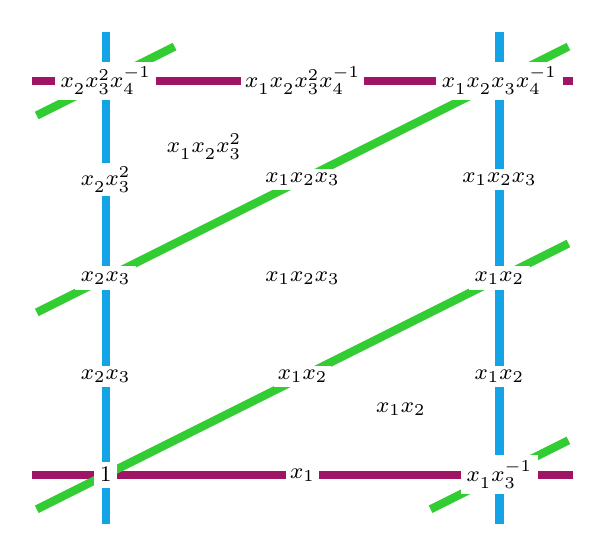
\begin{tikzpicture}[xscale=1.25, yscale=1.25, line width=3pt]
  \usetikzlibrary{calc, decorations.pathreplacing,shapes.misc, arrows.meta}
  \usetikzlibrary{decorations.pathmorphing}
  
  \tikzstyle{fuzz}=[RedViolet]%,
  \tikzstyle{fuzzB}=[Cerulean]%, 
  \tikzstyle{fuzzP}=[LimeGreen]%, 
 
  
  \coordinate  (origin) at (0,0);
  \coordinate (br) at (4,0);
  \coordinate (tr) at (4,4);
  \coordinate (tl) at (0,4);
  \coordinate (ml) at (0,2);
  \coordinate (mr) at (4,2);
  
  % Horizontal Edges
  \coordinate (hoff) at (0.75,0); %This seems like the wrong way to do it, but it works
  \draw[RedViolet] ($(origin)-(hoff)$) -- ($(br)+(hoff)$);
  \draw[RedViolet] ($(tl)-(hoff)$)--($(tr)+(hoff)$);
  % Use RedViolet instead of red

  % Vertical Edges
  \coordinate (voff) at (0,0.5);
  \draw[Cerulean] ($(origin)-(voff)$) -- ($(tl)+(voff)$);
  \draw[Cerulean] ($(br)-(voff)$) -- ($(tr)+(voff)$);
  % Use Cerulean instead of blue

  % Diagonal Edges
  \coordinate (diagoff) at (0.7,0.35);
  \draw[LimeGreen] ($(br)-(diagoff)$) -- ($(br)+(diagoff)$);
  \draw[LimeGreen] ($(origin)-(diagoff)$) -- ($(mr)+(diagoff)$);
  \draw[LimeGreen] ($(ml)-(diagoff)$) -- ($(tr)+(diagoff)$);
  \draw[LimeGreen] ($(tl)-(diagoff)$) -- ($(tl)+(diagoff)$);
  % Use LimeGreen instead of green

  %% Labels
  % points
  \node[inner sep = 2pt, fill=white] at (origin) {\footnotesize $1$};
  \node[inner sep = 2pt, fill=white] at (ml) {\footnotesize $x_2 x_3$};
  \node[inner sep = 2pt, fill=white] at (tl) {\footnotesize $x_2^{} x_3^2 x_4^{-1}$};
  \node[inner sep = 2pt, fill=white] at (br) {\footnotesize $x_1^{} x_3^{-1}$};
  \node[inner sep = 2pt, fill=white] at (mr) {\footnotesize $x_1 x_2$};
  \node[inner sep = 2pt, fill=white] at (tr)
  {\footnotesize $x_1^{} x_2^{} x_3^{} x_4^{-1}$};

  % edges
  \begin{scope}[inner sep = 1.5pt]
    % horizontal
    \node[fill=white] at ($(origin)!0.5!(br)$) {\footnotesize $x_1$};
    \node[fill=white] at ($(tl)!0.5!(tr)$) {\footnotesize
      $x_1^{} x_2^{} x_3^2 x_4^{-1}$};
    % vertical
    \node[fill=white] at ($(origin)!0.5!(ml)$) {\footnotesize $x_2x_3$};
    \node[fill=white] at ($(ml)!0.5!(tl)$) {\footnotesize $x_2^{} x_3^2$};
    \node[fill=white] at ($(br)!0.5!(mr)$) {\footnotesize $x_1 x_2$};
    \node[fill=white] at ($(mr)!0.5!(tr)$) {\footnotesize $x_1 x_2 x_3$};
    % diagonal
    \node[fill=white] at ($(origin)!0.5!(mr)$) {\footnotesize $x_1 x_2$};
    \node[fill=white] at ($(ml)!0.5!(tr)$) {\footnotesize $x_1 x_2 x_3$};
    
    % faces
    \node[fill=white] at (3,2/3) {\footnotesize $x_1 x_2$};
    \node[fill=white] at (2,2) {\footnotesize $x_1 x_2 x_3$};
    \node[fill=white] at (1,10/3) {\footnotesize $x_1^{} x_2^{} x_3^2$};
  \end{scope}
\end{tikzpicture}
$$
Here the lattice $L\subset M$ is given by:
$$
\begin{pmatrix}
 1&0\\
 0&1\\
 -1&2\\
 0&1
\end{pmatrix}: L = \ZZ^{2} \to M = \ZZ^{4}.
$$

\subsection{Acyclicity}

Since we are going to work on $\RR L/L$, we choose a fundamental domain for the action of $L$; in the case above it is given by square defined by the red and blue lines (note that in the quotient the red lines are identified, as are the blue lines).

In the construction of the Koszul complex, we stratified the free modules in the 
Koszul complex by divisibility.  In this case we stratify by the divisibility of the 
monomials $\Psi(p)$. Acyclicity is proven using \cite[Proposition 2.13]{BCHSY],} which says that if, for each $u\in M$ the set 
$$
\{ p\in \RR L \mid \Psi(p) divides u\}
$$
is acyclic and in this case the homogenized chain complex derived from the cellular
subdivision of $\RR L$ is a resolution of the momonomial module
$$
 X := S\cdot \{x^{\Psi(p)} \mid \p\in \RR L\}.
$$

\bibliographystyle{amsalpha}
\bibliography{Bibliography}

\end{document}
